\documentclass{article}

\usepackage[letterpaper]{geometry}
\usepackage{amsmath}
\usepackage{amssymb}
\usepackage{siunitx}
\usepackage{graphicx}

\title{4125 HW 1}
\author{Duncan Wilkie}
\date{27 January 2022}

\begin{document}

\maketitle

\section*{1.6}
If one touches a metal object that has been in contact with a temperature-regulated room's air for a very, very long time, it will feel colder to the touch than a book cover that has been in contact with the same air of the room for just as long. Intuitively, one feels that metals conduct heat better than the book, so one might conjecture your touch estimates temperature by the rate of change in your skin's energy, so that the room-temperature, thermally conductive object which removes your skin's heat faster feels colder than the less thermally conductive one at the same temperature. This will be generally right, since when touching the same material at different temperatures one might expect the colder one to remove energy faster.

\section*{1.7a}
The bulb at the bottom of the mercury thermometers we used in AP chemistry were about a centimeter in diameter. They therefore would have contained a volume of mercury
\[V=\frac{4}{3}\pi r^3=\frac{4}{3}\pi(\SI{5}{mm})^3=\SI{523.6}{mm^3}\]
If the temperature increases \SI{100}{K}, the volume increases by a factor of
\[\frac{\Delta V}{V}=\beta\Delta T=(\SI{1.81E-4}{K^{-1}})(\SI{100}{K})=0.0181\]
At this volume, that equates to
\[\Delta V=0.0181(\SI{523.6}{mm^3})=\SI{9.48}{mm^3}\]
Those same thermometers were about arm's length, but went to something like \SI{200}{^\circ C}, so I'll estimate the length between the \SI{0}{^\circ C} and \SI{100}{^\circ C} marks as \SI{0.15}{m}. A cylinder with this length and the above volume must have diameter according to
\[V=\pi r^2h\Rightarrow r=\sqrt{\frac{V}{\pi h}}=\sqrt{\frac{\SI{9.48}{mm^3}}{\pi(\SI{150}{mm})}}=\SI{0.142}{mm}\]
\[\Rightarrow d=\SI{0.284}{mm}\]
\section*{1.7b}
If the thermal expansion coefficient of water were always positive, the layer of water at the surface would cool down and become smaller, i.e. more dense. This would cause it to be negatively buoyant in comparison to the water below it, so the cold layer would tend to sink past those warmer layers and collect at the bottom. This would result in a persistent thermal gradient with the warmest water exposed to the cold surface air and the coldest on the bottom (I'm almost certain there's a simple differential equation that'd model the temperature gradient as a function of height, but that's a little too technical for this question). The average temperature of the lake continues to drop as the warm layer releases energy to the cold air, and eventually the average temperature would drop so low that the thermal gradient function with that average temperature would yield a bottom temperature below freezing. With no shortage of nucleation sites at the bottom, the whole lake would then start to freeze from the bottom up, killing any macroscopic aquatic life in the lake resembling that we see today.

\section*{1.10}
Take an average-sized room to have volume
\[\SI{7}{m}\times\SI{7}{m}\times\SI{3}{m}=\SI{147}{m^3}\]
Room temperature is \SI{300}{K}, and the pressure is of course $\SI{1}{atm}=\SI{1E5}{Pa}$, so by the ideal gas law
\[PV=nkT\Leftrightarrow n=\frac{PV}{kT}=\frac{(\SI{1E5}{Pa})(\SI{147}{m^3})}{(\SI{1.38E-23}{J/K})(\SI{300}{K})}=\SI{3.55E27}{molecules}\]

\section*{1.11}
Suppose the door were closed. Then room $A$ would have a higher pressure, because the volume of the room and the number of molecules of air in it are fixed and the temperature is greater. Therefore, when the door is opened the molecules in room $A$ will have a tendency to move into room $B$ to equalize the pressure, so room $B$ will have a greater number of them at equilibrium, and therefore a greater mass of air.

\section*{1.16a}
Let $h=dz$ and write the pressure balance the mathematical way (not 100\% competent with differential manipulations; I'll make fewer mistakes this way):
\[P(z-h/2)=P(z+h/2)+\rho hg\Leftrightarrow -\frac{P(z+h/2)-P(z-h/2)}{h}=\rho g\]
As $h\to 0$,
\[\frac{dP}{dz}=-\rho g\]
Writing Newton's second law in terms of pressures is justified because the force law is just the above equation multiplied through by the same factor: the area of the layer of air.

\section*{1.16b}
Noting that by definition $\rho V=mn \Leftrightarrow V=\frac{mn}{\rho}$, we may write the ideal gas law
\[PV=nkT\Leftrightarrow \frac{mnP}{\rho}=nkT\Leftrightarrow \rho = \frac{mP}{kT}\]
Plugging this in for $\rho$ in the result of part (a),
\[\frac{dP}{dz}=-\frac{mg}{kT}P\]
as desired.

\section*{1.16c}
This is a trivial case of separation of variables:
\[\frac{dP}{P}=-\frac{mg}{kT}dz\Leftrightarrow \ln P=-\frac{mg}{kT}z+c_0\Leftrightarrow P(z)=P_0\exp\left( -\frac{mg}{kT}z \right)\]
Applying the formula for density derived above,
\[\rho=\frac{mP_0}{kT}\exp\left( -\frac{mg}{kT}z \right)\]

\section*{1.16d}
The mass of an average air molecule can be found by a weighted average of the atomic weights of the molecules air is made up of by their relative abundances; from the problem cited and the table at the back of the book,
\[m=0.78\textrm{N}_2+0.21\textrm{O}_2+0.01\textrm{Ar}=0.78(\SI{28}{u})+0.21(\SI{32}{u})+0.01(\SI{39.95}{u})\]
\[=\SI{28.96}{u}=\SI{4.81e-26}{kg}\]
The temperature we assumed to be constant and can estimate to be \SI{300}{K}; the pressures are then
\[P_{Ut}=P_0\exp\left( -\frac{mg}{kT}z \right)=(\SI{1}{atm})\exp\left( -\frac{(\SI{4.81E-26}{kg})(\SI{9.81}{m/s^2})}{(\SI{1.38E-23}{J/K})(\SI{300}{K})}(\SI{1430}{m}) \right)=\SI{0.8496}{atm}\]
\[P_{Co}=P_0\exp\left( -\frac{mg}{kT}z \right)=(\SI{1}{atm})\exp\left( -\frac{(\SI{4.81E-26}{kg})(\SI{9.81}{m/s^2})}{(\SI{1.38E-23}{J/K})(\SI{300}{K})}(\SI{3090}{m}) \right)=\SI{0.703}{atm}\]
\[P_{Ca}=P_0\exp\left( -\frac{mg}{kT}z \right)=(\SI{1}{atm})\exp\left( -\frac{(\SI{4.81E-26}{kg})(\SI{9.81}{m/s^2})}{(\SI{1.38E-23}{J/K})(\SI{300}{K})}(\SI{4420}{m}) \right)=\SI{0.604}{atm}\]
\[P_{Ev}=P_0\exp\left( -\frac{mg}{kT}z \right)=(\SI{1}{atm})\exp\left( -\frac{(\SI{4.81E-26}{kg})(\SI{9.81}{m/s^2})}{(\SI{1.38E-23}{J/K})(\SI{300}{K})}(\SI{8840}{m}) \right)=\SI{0.365}{atm}\]

\section*{1.22a}
The pressure is the average force per unit area resulting from the collisions of the molecules with the wall of the container. The per-collision impulse is $2m\overline{v_x}$ by assumption of elasticity; in terms of the number of collisions $n$ with $A$ over $\Delta t$, the average force on $A$ is by the definition of impulse $\overline{F}=\frac{n(2m\overline{v_x})}{\Delta t}$. Therefore, the pressure on the surface $A$ is.
\[P=\frac{\overline{F}}{A}=\frac{2nm\overline{v_x}}{A\Delta t}\]
Plugging this form of pressure into the desired expression, we can verify that it does in fact reduce to $n$:
\[\frac{PA\Delta t}{2m\overline{v_x}}=\frac{2nm\overline{v_x}}{A\Delta t}\frac{A\Delta t}{2m\overline{v_x}}=n\]
as desired.

\section*{1.22b}
This is derived in the book, so I don't know why it's an exercise. In any case, consider a single molecule in the container; the average pressure on the wall of the container is the force on the container divided by the area of the wall. The force on the molecule is the negation of the force on the container by Newton's third law, i.e.
\[\overline{P}=-\frac{\overline{F_x}}{A}=-\frac{m\overline{\frac{\Delta v_x}{\Delta t}}}{A}\]
To minimize the error in treating the discrete process like a continuous one, the longer time interval the better, since this will allow more collisions of the molecules with the wall and make the ``sample'' changes in the velocities close to the ``population'' changes in velocities. However, if the molecule is allowed to hit the other side of the container that results in another force not captured in the above equation, so the most accurate expression for the time difference will be such that the particle starts at the far side, bounces off the near side, and returns:
\[\Delta t=\frac{2L}{v_x}\]
The expression  $\Delta v_x=-2v_x$ follows from the collision being elastic, so
\[\overline{P}=-\frac{m\frac{-2v_x}{2L/v_x}}{A}=\frac{mv_x^2}{AL}=\frac{mv_x^2}{V}\Rightarrow \overline{P}{V}=mv_x^2\]
With very many particles making up an ideal gas, the right-hand side of the above equation accumulates an additional term identical except for having a different velocity for each new particle; writing this sum in terms of the average value of $v_x^2$ over the particles and presuming the pressure to be virtually constant, we have
\[PV=Nm\overline{v_x^2}\]
However, the ideal gas law states $PV=NkT$; equating the right-hand sides of the two equations, we obtain
\[Nm\overline{v_x^2}=NkT\Leftrightarrow \sqrt{\overline{v_x^2}}=\sqrt{\frac{kT}{m}}\]
as desired.

\section*{1.22c}
Over a time interval $dt$, the change in the number of molecules $dN$ is given by the (negative of the) formula derived in (a). Estimating $\overline{v_x}$ by $\sqrt{\overline{v_x^2}}$ using the result from (b),
\[dN=-\frac{PAdt}{2m\sqrt{kT/m}}\]
Using $PV=NkT\Leftrightarrow P=\frac{NkT}{V}$,
\[\frac{dN}{dt}=-\frac{NkTA}{2mV\sqrt{kT/m}}=-\frac{A}{2V}\sqrt{\frac{kT}{m}}N\]
as desired. This may be solved very simply by separation of variables:
\[\frac{dN}{N}=-\frac{A}{2V}\sqrt{\frac{kT}{m}}dt\Leftrightarrow N(t)=N_0\exp\left( -\frac{A}{2V}\sqrt{\frac{kT}{m}}t \right)\]
The characteristic time is
\[\tau=\frac{2V}{A}\sqrt{\frac{m}{kT}}\]

\section*{1.22d}
We assume $T=\SI{300}{K}$ and an average molecular mass of air, $\SI{4.81e-26}{kg}$.
\[\tau=\frac{2V}{A}\sqrt{\frac{kT}{m}}=\frac{2(\SI{0.001}{m^3})}{\SI{1e-6}{m^2}}\sqrt{\frac{\SI{4.81e-26}{kg}}{(\SI{1.38e-23}{J/K})(\SI{300}{K})}}=\SI{4.056e-4}{s}\]

\section*{1.22e}
We presume $\SI{300}{K}$, and a \SI{1}{L} tire. The bicycle tire may be called flat when only a quarter or so of the initial molecules remain. The corresponding number of time constants that must have elapsed is $-\ln(0.25)=1.386$, i.e. $\SI{1}{hr}=1.386\tau\Rightarrow \tau=\frac{1}{1.386}=\SI{0.721}{hr}=\SI{2596}{s}$.
Solving the time constant expression for $A$,
\[A=\frac{2V}{\tau}\sqrt{\frac{m}{kT}}=\frac{2(\SI{0.001}{m^3})}{\SI{2596}{s}}\sqrt{\frac{\SI{4.81e-26}{kg}}{(\SI{1.38e-23}{J/K})(\SI{300}{K})}}=\SI{2.626e-9}{m^2}=\SI{0.0023}{mm^2}\]

\section*{1.22f}
Presuming \SI{300}{K}, a half-second opening period, a \SI{10}{m^3} spacecraft, and a \SI{1}{m^2} window, the proportion of the initial atmosphere remaining would be
\[\exp\left(-\frac{A}{2V}\sqrt{\frac{kT}{m}}t \right)=\exp\left(- \frac{\SI{1}{m^3}}{2(\SI{10}{m^3})}\sqrt{\frac{(\SI{1.38e-23}{J/K})(\SI{300}{K})}{\SI{4.81e-26}{kg}}}(\SI{0.5}{s}) \right)={6.53}\times10^{-4}\]
\[=0.0653\%\]
I don't believe that's survivable.

\section*{1.25}
The water molecule $\textrm{H}_2\textrm{O}$ has a bond angle of $120^\circ$, with the oxygen as the base point. This results in:
\begin{itemize}
\item Three translational degrees of freedom of the whole atom in free space
\item Three rotational degrees of freedom of the whole atom about each of the axis (if the bond were linear, one would vanish, but it isn't)
\item Two linear vibrational degrees of freedom of each of the bonds along their length
\item Four angular vibrational degrees of freedom from each of the bonds' angular displacement in the spherical coordinate system originating at the oxygen atom
\end{itemize}

\section*{1}
We have $\SI{50}{^\circ Fl}=\SI{44}{^\circ C}+273=\SI{317}{K}$ and $\SI{0}{^\circ Fl}=\SI{-18.75}{^\circ C}+273=\SI{254.25}{K}$. Taking the ratio of the changes in the scales,
\[\frac{\Delta K}{\Delta ^\circ Fl}=\frac{\SI{317}{K}-\SI{254.25}{K}}{\SI{50}{^\circ Fl}}=\SI{0.0159}{K/^\circ Fl}\]
The initial temperature corresponds to the \SI{0}{^\circ Fl} number given above, so the formula is
\[K=0.0159(^\circ Fl)+254.25\]
The conversion from Kelvin to Fahrenheit is
\[^\circ F=\frac{9}{5}K-459.67\]
Composing this formula with the above yields the Florentine to Fahrenheit formula
\[^\circ F=\frac{9}{5}(0.0159(^\circ Fl)+254.25)-459.67=0.0287(^\circ Fl)-2.02\]

\section*{2}
The given volume curve is shown below via gnuplot.
\[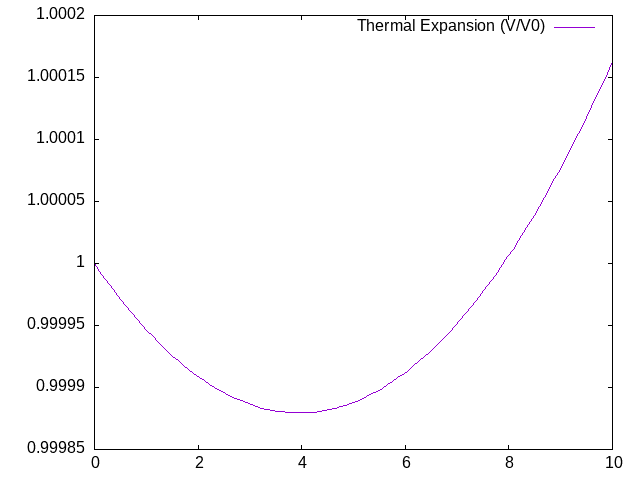
\includegraphics[scale=.5]{img.png}\]
Consider starting the thermometer at the minimum around \SI{4}{^\circ C}. Increasing or decreasing the real temperature by the same amount would result in the same temperature reading, up to about a \SI{4}{^\circ C} displacement in each direction about the vertex. As a result, the thermometer is essentially useless at these temperatures.

\end{document}
%%% Local Variables:
%%% mode: latex
%%% TeX-master: t
%%% End:
